\documentclass[output=paper,colorlinks,citecolor=brown]{langscibook}
\ChapterDOI{10.5281/zenodo.15654863}
\title{Reassessing Oehrle effects: Evidence from Scottish Gaelic}
\author{Gary Thoms\affiliation{New York University}}

\IfFileExists{../localcommands.tex}{
   % add all extra packages you need to load to this file

\usepackage{tabularx,multicol}
\usepackage{url}
\urlstyle{same}

\usepackage{listings}
\lstset{basicstyle=\ttfamily,tabsize=2,breaklines=true}

\usepackage{langsci-basic}
\usepackage{langsci-optional}
\usepackage{langsci-lgr}
\usepackage{langsci-osl}
% \usepackage{./langsci/styles/langsci-lgr}
% \usepackage{./langsci/styles/langsci-osl}
% \usepackage{langsci-gb4e}

\usepackage{tikz}
\usetikzlibrary{patterns,calc}
\pgfdeclarepatternformonly{south east lines}{\pgfqpoint{-0pt}{-0pt}}{\pgfqpoint{3pt}{3pt}}{\pgfqpoint{3pt}{3pt}}{
    \pgfsetlinewidth{0.6pt}
    \pgfpathmoveto{\pgfqpoint{0pt}{3pt}}
    \pgfpathlineto{\pgfqpoint{3pt}{0pt}}
    \pgfpathmoveto{\pgfqpoint{.2pt}{-.2pt}}
    \pgfpathlineto{\pgfqpoint{-.2pt}{.2pt}}
    \pgfpathmoveto{\pgfqpoint{3.2pt}{2.8pt}}
    \pgfpathlineto{\pgfqpoint{2.8pt}{3.2pt}}
    \pgfusepath{stroke}}
    
\usepackage{stmaryrd}
\usepackage{wasysym}
\usepackage{multirow}
\usepackage{caption}
\usepackage{subcaption}
\usepackage{mathrsfs}
\usepackage{qtree}

\usepackage{linguex}


   %pminos do not split footnotes
% \interfootnotelinepenalty=10000 %Footnote in Laporte chapters has to be split SN


%\DeclareIndexNameFormat{default}{%
%\nameparts{#1}%
%\usebibmacro{index:name}%
%{\index[names]}%
%{\namepartfamily}%
%{\namepartgiveni}%
% {}% L1
% {}% L2
%{\namepartprefix}% generates spurious space L3
%{\namepartsuffix}% generates spurious space L4
%}

%  {\DeclareIndexNameFormat{default}{%
%     \usebibmacro{index:name}{\index[names]}{#1}{#3}{#5}{#7}}}

%\DeclareIndexNameFormat{default}{%
%  \usebibmacro{index:name}{\sindex[nom]}{#1}{#3}{#5}{#7}}

%\DeclareIndexNameFormat{default}{%
%  \usebibmacro{index:name}{\sindex[person]}{#1}{#3}{#5}{#7}}
%\DeclareIndexNameFormat{default}{%
%\nameparts{#1} \usebibmacro{index:name}{\sindex[person]]}{\namepartfamily}{‌​\namepartgiven}{\nam‌​epartprefix}{\namepa‌​rtsuffix}}

%\newcommand{\smiley}{:)}

%\renewbibmacro*{index:name}[5]{%
%\usebibmacro{index:entry}{#1}%
%{\iffieldundef{usera}{}{\thefield{usera}\actualoperator}\mkbibindexname{#2}{#3}{#4}{#5}}}

% \newcommand{\noop}[1]{}

%remove for final
%\overfullrule=1mm

\newcommand{\tobi}[2]}}
\renewcommand{\S}[1]{\tobi{#1}{\textsc{*}}}

% this volume references
% puts: [this volume]
% already defined: \citetv
%\newcommand{\citepv}[1]{(\citeauthor{#1} \citeyear*{#1} [this volume])}
\newcommand{\citealtv}[1]{\citeauthor{#1} \citeyear*{#1} [this volume]}

%parentheses around example number
\newcommand{\pref}[1]{(\ref{#1})}

% in-text examples

\newcommand{\lnex}[1]{\textit{#1}} %target lang word
\newcommand{\lnlit}[1]{(lit.: `#1')} %literal reading
\newcommand{\lnlat}[1]{(#1)} % latinization
\newcommand{\lntrans}[1]{`#1'} %translation
\newcommand{\lnexl}[2]%
{\lnex{#1}{} \lnlat{#2}} % ex with latinization
\newcommand{\lnexlat}[3]{\lnex{#1}{} \lnlat{#2}{} \lntrans{#3}} % ex with latinization and tranl.

%ch01
\newcommand{\co}[1]{\mbox{\textbf{#1}}}

%ch09

\newcommand{\cyrbulg}[1]{\begin{otherlanguage*}{bulgarian}#1\end{otherlanguage*}}


%ch10
\newcommand{\nlp}{{\small NLP}}
\newcommand{\mwe}{{\small MWE}}
\newcommand{\rae}{{\small RAE}}
\newcommand{\lvc}{{\small LVC}}
\newcommand{\pos}{{\small P}o{\small S}}
%\newcommand{\todo}[1]{ \textcolor{red}{#1} }

%\renewcommand{\labelenumi}{\theenumi}
%\ainamefmt{{vv}{ll}{, ff}{, jj}} % fullname

\newcommand{\biberror}[1]{{\color{red}#1}}

\newcommand{\osenovaitem}{--~}
   %% hyphenation points for line breaks
%% Normally, automatic hyphenation in LaTeX is very good
%% If a word is mis-hyphenated, add it to this file
%%
%% add information to TeX file before \begin{document} with:
%% %% hyphenation points for line breaks
%% Normally, automatic hyphenation in LaTeX is very good
%% If a word is mis-hyphenated, add it to this file
%%
%% add information to TeX file before \begin{document} with:
%% %% hyphenation points for line breaks
%% Normally, automatic hyphenation in LaTeX is very good
%% If a word is mis-hyphenated, add it to this file
%%
%% add information to TeX file before \begin{document} with:
%% \include{localhyphenation}
\hyphenation{
    Beck-man
    Ngu-yen
    back-chan-nel
    back-chan-nels
    mo-not-o-nous
    ste-reo-typ-i-cal
}

\hyphenation{
    Beck-man
    Ngu-yen
    back-chan-nel
    back-chan-nels
    mo-not-o-nous
    ste-reo-typ-i-cal
}

\hyphenation{
    Beck-man
    Ngu-yen
    back-chan-nel
    back-chan-nels
    mo-not-o-nous
    ste-reo-typ-i-cal
}

   \boolfalse{bookcompile}
   \togglepaper[4]%%chapternumber
   \pgfplotsset{compat=1.18}
}{}

\AffiliationsWithoutIndexing



\abstract{It has often been argued that the double object construction and prepositional dative construction differ semantically -- in particular, that the double object construction has a possessive core which is not shared by the prepositional dative -- on the basis of various cases where the dative alternation breaks down in languages such as English. These ``Oehrle effects'' have been argued to support a two-base analysis of the dative alternation (e.g., \cite{gt:Harley:2002a}) over derivational accounts (e.g., \cite{gt:Larson:1988}). This article counters this argument on the basis of data from Scottish Gaelic, which expresses ditransitives exclusively in terms of prepositional datives. It is shown that Oehrle effects do not obtain in this language: various ditransitive types which resist the prepositional dative in alternating languages do not show any such resistance to the frame in Scottish Gaelic, a fact that tells us that the problem behind Oehrle effects cannot be one of semantic incompatibility. I provide an alternative syntactic account of Oehrle effects in English\il{English (Modern)} and their absence in Scottish Gaelic, arguing that they can be explained in terms of the height of certain subject arguments and their interaction with object shift operations, which vary from language to language. }

%\usepackage{tabularx}
%\usepackage{langsci-optional}
%\usepackage{langsci-gb4e}
%\usepackage{color}
%\usepackage{comment}
%\usepackage{tikz-qtree,tikz-qtree-compat,pifont}
%
%
%\bibliography{localbibliography}
%
%
%%\bibliography{lingbib4}
%\newcommand{\orcid}[1]{}
%\newcommand{\tb}[1]{\textbf{#1}}
%\newcommand{\cat}[1]{$_{\textsc{\scriptsize #1}}$}

%\usetikzlibrary{positioning}
%   
%   \usetikzlibrary{arrows.meta}
%   
%\tikzset{exarrows/.style={semithick,
%                             arrows={-Stealth[scale=1, scale length=1,
%                                              scale width=1]}}}

\begin{document}

\maketitle

\il{Irish (Modern)|(}
\il{Scottish Gaelic (Modern)|(}
\il{Gaelic|see{Scottish Gaelic (Modern)}}

\section{Introduction}

In  Scottish Gaelic and Irish, ditransitives are expressed exclusively in the form of prepositional dative constructions (PDCs), as in (\ref{a2}--\ref{a1}), where the indirect object (IO; the goal/recipient) is marked with a preposition and preceded by an unmarked direct object (DO; theme) in neutral word order.

\xe{a2}{
\gll Thug M\`airi leabhar do dh'Iain.  \\
give.\textsc{pst} Mairi book to Iain  \\
\glt `Mairi gave a book to Iain.'  \hfill (SG) }

\xe{a1}{
\gll Thug M\'aire leabhar do She\'an. \\
give.\textsc{pst} Maire book to Sean  \\
\glt `Maire gave a book to Sean.' \hfill (Irish)}

\noindent Most theoretical analyses of PDCs in the literature have centered on the question of whether they are related to double object constructions (DOCs), in particular in languages such as English\il{English (Modern)} that show an alternation between the two, known as the dative alternation. In one family of analyses, the two constructions are taken to be derivationally related, and one of the two structures forms the base for construction of the other; we can call this the \eee{derivational theory} (\citealt{gt:Larson:1988}; \citealt{gt:Snyder:1997}; \citealt{gt:Ormazabal:2012}, \citeyear {gt:Ormazabal:2023}; \citealt{gt:Collins:2023}; cf. also \citealt{gt:Rappaport:2008}). In another family of analyses, which \citet{gt:Harley:2017} identify as being representative of a ``relatively broad consensus'', the two constructions are distinct argument structures altogether with different base positions for the arguments; call this the \eee{two-base theory} (\citealt{gt:Green:1974}; \citealt{gt:Oehrle:1976}; \citealt{gt:Marantz:1993}; \citealt{gt:Pesetsky:1995}; \citealt{gt:Pylkkanen:2002a}, \citeyear{gt:Pylkkanen:2008}; \citealt{gt:Harley:2002a}; \citealt{gt:Harley:2015}; \citealt{gt:Bruening:2001a}, \citeyear{gt:Bruening:2010a}, \citeyear{gt:Bruening:2010b}, \citeyear{gt:Bruening:2018a}).  The debate between these two theories speaks to a number of major theoretical issues, such as the status of Baker's Uniformity of Theta Assignment Hypothesis (UTAH): in essence, UTAH predicts that some version of the single-base theory must be right; it would, in its strongest form, rule out the two-base theory altogether. The debate has largely centered on alternating languages such as English\il{English (Modern)}, while relatively little attention has been paid to PDC-only languages such as Scottish Gaelic and Irish. 
 
One of the main sources of debate is the proper treatment of cases where the dative alternation breaks down, as in (\ref{gt:m6}--\ref{gt:he1}), or where the two frames seem to give rise to different interpretations, as in (\ref{gt:m3}). Many such cases were first identified in English\il{English (Modern)} by Oehrle (\citeyear{gt:Oehrle:1976}; but see also \citealt{gt:Green:1974}), and they have often been described as ``Oehrle effects''.\is{Oehrle effect}

\xex{gt:m6}{ 
\xl{gt:m6a} The editor sent the article to Philadelphia. 
\xl{gt:m6b} *The editor sent Philadelphia the article.} 

\xex{gt:in1}{
\xl{gt:in1a} The war years gave Mailer a book. 
\xl{gt:in1b} *The war years gave a book to Mailer. }

\protectedex{
\xex{gt:he1}{
\xl{gt:he1a} The lighting here gives me a headache. 
\xl{gt:he1b} *The lighting here gives a headache to me.  \hfill (\cite[288]{gt:Bruening:2010a})}
}

\xex{gt:m3}{
\xl{gt:m3a} John gave Mary a child. \hfill \eee{can mean} `John got Mary pregnant'
\xl{gt:m3b} John gave a child to Mary.  \hfill \eee{can't mean} `John got Mary pregnant' \newline \phantom{cc} \hfill (\cite[42]{gt:Harley:2002a})}

\noindent A common analysis of these pairs is that they show that the DOC and PDC have distinct meanings: DOCs have a \textsc{caused possession} interpretation, whereby the indirect object (IO) becomes the possessor of the direct object (DO), while PDCs don't involve caused possession but rather some event involving an agent, a theme, and a goal that is introduced by a preposition. Ditransitives of the kind in (\ref{gt:m6}--\ref{gt:m3}) allow us to see this difference, it's claimed, because one or the other of their arguments is semantically incompatible with the relevant thematic roles; for example, the IO in (\ref{gt:m3}) must be a true possessor for the intended (inalienable) interpretation.\footnote{\label{gt:fnn}This reading seems somewhat archaic for many speakers, but a similar effect can be demonstrated with \eee{John and Mary gave their parents a beautiful grandchild}, which is less archaic and also fails as a PDC on the right interpretation (\eee{*John and Mary gave a beautiful grandchild to their parents}).} This account makes a clear prediction, mentioned by \citet[66, fn. 12]{gt:Harley:2002a}: in languages that don't have access to the DOC at all, such as the Celtic languages, we should find that the Oehrle effect cases -- those ditransitive types that are specific to DOCs, such as (\ref{gt:in1}--\ref{gt:m3}) above -- are simply inexpressible with the language's ditransitives because the PDC frame is semantically incompatible with such caused possession meanings. 

In this chapter, I show that this prediction is not borne out: PDCs in non-alternating languages such as Scottish Gaelic don't show any of the supposedly semantic restrictions that English\il{English (Modern)} PDCs show. It can be concluded that the English\il{English (Modern)} contrasts should not be explained in terms of semantic distinctions between the frames but rather in terms of some other, most likely syntactic, ingredients of the ditransitive frames. With the semantic explanation put to one side, I develop an alternative syntactic analysis of Oehrle effects\is{Oehrle effect}, attributing the relevant effects to the interaction of \isi{object shift} and low non-agentive subjects. The differences between English\il{English (Modern)} and Scottish Gaelic that are documented with respect to Oehrle effects\is{Oehrle effect} are then tied to differences in the distribution of object positions in the languages. The resulting picture is one where the apparently semantic constraints on PDCs are given a thoroughly syntactic reappraisal. 

\section{On the two-base theory}

The leading idea in \citet{gt:Harley:2002a} is that ditransitives involve a causative light verb embedding a small clause-like structure which is headed by a preposition, and the preposition introduces one argument in its complement domain and another in its specifier. The two argument structure frames involve the use of different abstract prepositions which have distinct but largely overlapping meaning contributions, and they are taken to be related to the structures involved in different kinds of possessive predication crosslinguistically. For DOCs, the preposition is identified with the P that \citet{gt:Kayne:1993} took to be at the core of \textsc{have}-possessives -- hence it is called  P$_{\textsc{have}}$ -- and it takes a DP as its complement. This is in \figref{have}a. For PDCs, the preposition has a locative semantics -- hence it is called P$_{\textsc{loc}}$ -- and it takes a PP as its complement. This preposition, Harley claims, is akin to the one that is involved in negotiating predicative possession relations in \textsc{be}-possessive languages, such as Irish and Scottish Gaelic. This is in \figref{have}b. 

\begin{figure}[h]
\caption{Harley's structures for DOCs (a) versus PDCs (b)}
\label{have}
\begin{subfigure}{.5\textwidth}
\centering
\begin{forest}
    [\textit{v}P [DP][\textit{v}[v\textsubscript{CAUSE}][PP [DP][P$'$ [P\textsubscript{HAVE}][DP] ]]]]
\end{forest}
\caption{}
\end{subfigure}\begin{subfigure}{.5\textwidth}
\centering
\begin{forest}
    [\textit{v}P [DP][\textit{v}[v\textsubscript{CAUSE}][PP [DP][P$'$ [P\textsubscript{LOC}][PP]]]]]
\end{forest}
\caption{}
\end{subfigure}
\end{figure}

Harley's account captures contrasts such as (\ref{gt:m6}--\ref{gt:he1}) quite straightforwardly. (\ref{gt:m6}) follows because ``Philadelphia'' can be a location or goal but not a possessor (cf.\ \eee{\#Philadelphia has the letter}), whereas (\ref{gt:in1} and \ref{gt:he1}) hold because the predications involve some sort of caused possession (e.g.\ \ref{gt:he1a} is paraphrasable as ``the lighting caused me to have a headache''); however, the IOs are not locations or goals in any real sense.

Harley's analysis generalizes to other cases of failed PDCs where the IO is not plausibly a location or goal, whereas it could be a possessor in the associated DOC, as is the case with \eee{cost} and \eee{spare} (\ref{gt:ac1}--\ref{gt:cc1}), both of which have negative caused possession interpretations of some sort (``cause to not have''). 

\xex{gt:ac1}{
\xl{c1a} That decision cost John a job. 
\xl{c1b} *That decision cost a job to John. }

\xex{gt:cc1}{
\xl{gt:cc1a} They spared me that ordeal. 
\xl{gt:cc1b} *They spared that ordeal to me. }

\noindent It may also capture some effects noted by \citet[157]{gt:Green:1974} regarding the interpretation of the ditransitive use of \eee{teach} as in (\ref{m1}), where it is claimed that while the DOC in (\ref{m1a}) has the implication that the students ended up learning (`having') some French, the PDC in (\ref{m1b}) lacks this implication. Although the effect in (\ref{m1}) is weak or nonexistent for some speakers or in certain configurations,\footnote{See \citet[144--150]{gt:Rappaport:2008} for discussion of this specific example, and also the general question of whether DOCs and PDCs really do differ systematically with respect to successful transfer inferences.  } the caused possession interpretation is arguably more strongly required with cases such as (\ref{in22a}) with non-agentive causer subjects, where the corresponding PDCs (\ref{in22b}) are wholly unacceptable, as noted by \citet{gt:Oehrle:1976}. 

\xex{m1}{
\xl{m1a} John taught the students French.  
\xl{m1b} John taught French to the students.  }

\xex{in22}{
\xl{in22a} Lipson's textbook taught me Russian. 
\xl{in22b} *Lipson's textbook taught Russian to me. \hfill (\cite[193]{gt:Pesetsky:1995}) }

\noindent These effects should follow if the PDC lacks a caused possession interpretation, and instead its PP has a goal interpretation.

Another set of contrasts that Harley attributes to the two-base theory is the fact that many ditransitive idioms fail to alternate between one frame or another (see also \citealt{gt:Richards:2001}). (\ref{m4}--\ref{m5}) demonstrate two well-known examples. 


\xex{m4}{
\xl{m4a} Oscar will give John the boot. 
\xl{m4b} *Oscar will give the boot to John.  }

\xex{m5}{
\xl{m5a} Lasorda sent his starting pitcher to the showers.
\xl{m5b} *Lasorda sent the showers his starting pitcher.  }

\noindent Harley argues that such facts can be captured if the idioms involved correspond to stored  substructures of the distinct prepositional small clauses associated with the two frames. So, \eee{give X the boot} involves a P$_{\textsc{have}}$' idiom (comprising the P$_{\textsc{have}}$ head and its complement DP \eee{the boot}), and so (\ref{m4b}) is impossible because the PDC does not have P$_{\textsc{have}}$' as its substructure. Something similar is said to obtain with (\ref{m5a}), where the idiom involved is a P$_{\textsc{loc}}$ idiom which cannot be a subpart of a DOC, hence the impossibility of (\ref{m5b}). 

Subsequent incarnations of the two-base approach, such as Bruening (\citeyear{gt:Bruening:2010a}, \citeyear{gt:Bruening:2010b}) and \citet{gt:Harley:2015}, have maintained the same basic idea: the DOC involves a caused possession semantics whereas the PDC does not. Bruening argues against the ``symmetry'' of Harley's small clause analysis, and in favour of an analysis where DOCs are structurally more complex -- with an ApplP projection above VP encoding possessive semantics, whereas the PDC lacks this and, thus, the possessive interpretation. Most of the issues discussed in what follows present the same sort of challenges for this whole set of analyses; therefore, I focus on Harley's original proposal with some additional remarks clarifying differences with others. 

\section{Celtic and Oehrle effects}

\subsection{Celtic and the distribution of ditransitive frames}

The Celtic languages are all VSO languages whose ditransitives involve V-S-DO-IO order by default. In Scottish Gaelic, IOs can be introduced by various prepositions, but the most widely used ones are \eee{do} (plus lenition) `to' and \eee{gu} `to(wards)', the latter typically conveying a clearer sense of directed motion; compare (\ref{tr1}) with (\ref{tr2}). The light verb \eee{thoir} combines with either, giving rise to different translation equivalents in each case. (Henceforth, all non-English examples are Scottish Gaelic unless otherwise indicated.)

\xe{tr1}{ 
\gll Thug iad leabhraichean do dh'Iain. \\
give.\textsc{pst} they books to Iain \\
\glt `They gave books to Iain.' }

\xe{tr2}{
\gll Thug iad leabhraichean gu Iain. \\
give.\textsc{pst} they books to Iain \\
\glt `They brought books to Iain.' }

\noindent As noted, \eee{gu} `to(wards)' is typically used for verbs with a directed motion component, similar to \eee{cuir} in its `send' use (see \ref{dr3}--\ref{dr4a}), but a distinct preposition \eee{a} is used with locational goals. This is most likely a distinction akin to the dative/allative distinction, the relevance of which for the analysis of the \eee{send} contrasts is insightfully discussed in \citet{gt:Rappaport:2008}.  

\xe{dr3}{ 
\gll Chuir iad leabhraichean gu Iain. \\
send.\textsc{pst} they books to Iain \\
\glt `They sent books to Iain.' }

\xe{dr4a}{ 
\gll Chuir iad leabhraichean a Ghlaschu. \\
send.\textsc{pst} they books to Glasgow \\
\glt `They sent books to Glasgow.' }

\noindent Prepositions in these languages inflect for features of their complements, and pronominal complements are covert due to the well-known complementarity between head marking and pronominal expression we see in these languages. In what follows I simply gloss the P-pronoun amalgamations in the format `at.me' and `with-him' for ease of reading, with no concrete commitment on the specific analysis (on which see e.g., \citealt{gt:McCloskey:1984a}).  

\citet{gt:Harley:2002a} brought Celtic into the discussion in the ditransitive literature by way of a typological argument in favour of her theory. Having proposed P$_{\textsc{have}}$ as the crucial ingredient of DOCs, Harley identified the prediction that languages which lack a verbal \textsc{have} predicate will also lack DOCs, since both are based on P$_{\textsc{have}}$. She claimed that Irish and Scottish Gaelic bore this out, since they lack verbal \textsc{have} and also lack DOCs, as the examples in (\ref{do1}) show. 

\xex{do1}{
\xl{do1a} \gll *Thug M\'aire S(h)e\'an leabhar. \\
give.\textsc{pst} Maire Sean book  \\
\glt intended: `Maire gave Sean a book'  \hfill  (Irish, \citealt{gt:Jung:2012}) 
%
\xl{do1b} \gll *Thug Mairi (dh')Iain leabhar. \\
give.\textsc{pst} Mairi Iain book \\
\glt intended: `Mairi gave Iain a book.'  }

\noindent The Celtic languages express predicative possession with \textsc{be}-possessives that mark the possessor with an adposition. In Scottish Gaelic, the adposition is \eee{aig} `at', and the PP shows up after the possessee (\ref{rt1}). 

\xe{rt1}{ 
\gll Tha leabhar aig Iain. \\
be.\textsc{prs} book at Iain \\
\glt `Iain has a book.' \hfill } 

\noindent \citet{gt:Harley:2002a} claims that this constitutes an instance of the P$_{\textsc{loc}}$ small clause that is implicated in her analysis of the PDC.

However, there are some challenges for this analysis. One comes from the fact that the \textsc{be}-possessive clauses in Celtic seem to be very much possessive and not locative in their semantics. For example, they can be used to express inalienable possession relations of various kinds, as well as abstract possession, as the examples in (\ref{huv}) demonstrate for Scottish Gaelic.\footnote{Part-whole relations with inanimates are expressed with similar constructions but a different preposition, \eee{air} ``on''. 

\xe{huv2}{\gll Tha ceithir casan air a’ bhòrd. \\ 
be.\textsc{prs} four legs on the table \\
\glt `The table has four legs.' }

} 

\xex{huv}{
\xl{huv1} \gll Tha piuthar agam. \\
be.\textsc{prs} sister at.me\\
\glt `I have a sister.' (somewhere in the world) \label{sister}
%
\xl{huv3}\gll Tha sùilean gorma agam. \\
be.\textsc{prs} eyes blue at.me \\
\glt `I have blue eyes.' 
%
\xl{huv4} \gll Tha ceann goirt agam.\\
be.\textsc{prs} head sore at.me \\
\glt `I have a headache.' }

\noindent In fact, the language even uses the same construction for having knowledge of a language. If the PP argument of a P$_{\textsc{loc}}$ structure is a goal, as Harley claims, then it's hard to see how (\ref{gae}) could be well-formed whereas (\ref{in22b}) with \eee{teach} in the PDC could be bad. Recall, the latter was ruled out on the basis of the PP argument that represents the seat of imparted linguistic knowledge not making a good goal, yet by the same logic the PP in (\ref{gae}) would be the same sort of of goal.

\xe{gae}{
\gll Tha G\`aidhlig agam.  \\
be.\textsc{prs} Gaelic at.me \\
\glt `I know Gaelic', `I have Gaelic', lit. `Gaelic is at me'  }

\noindent If the language's PDCs and predicative possession clauses have common grammatical ingredients, one would not really expect the PDCs to be restricted to locative interpretations. 

Still, the relationship between the \textsc{be}-possessives and the PDCs must be at least a little abstract, because they involve different adpositions (\eee{aig} `a' with \textsc{be}-possessives,  \eee{do} and others in PDCs). Therefore, it is possible that these independent differences account for the difference between predicative possession and Scottish Gaelic PDCs with respect to their possessive interpretations. However, we still need to ascertain whether Scottish Gaelic PDCs do have a possessive interpretation when looking beyond the simple examples discussed so far. 

\subsection{Caused possession}

\citet[67, fn 12]{gt:Harley:2002a}  noted the specific prediction that the Celtic languages should not allow caused possession constructions of the type associated with Oehrle effects, saying ``[o]ne wonders if in Irish idiomatic/metaphoric expressions like \eee{The war years gave Mailer a book} are ill-formed; the current analysis seems to predict that they should be.'' Although this particular construction doesn't seem to arise in Scottish Gaelic,\footnote{This is paralleled to some degree by the facts from English\il{English (Modern)}; I have found that a reasonable number of speakers (including native-speaker linguists who are familiar with the issues) find these \eee{give X (the idea for) a book} uses of \eee{give} quite outside of their English\il{English (Modern)}. I have not investigated this variation in sufficient detail to rule out the possibility that there is some independent issue with these specific sentences. All of these speakers find a version of the DOC with \eee{an idea for a book} as the DO completely acceptable. } similar examples with caused possession of abstract DOs are possible, such as (\ref{mail}) and (\ref{dr5}). 

\xe{mail}{\gll Thug a bhliadhnaichean sa chogadh sealladh ùr dha. \\
gave his years in.the war outlook new to.him  \\
\glt `His years in the war gave him a new outlook.' (cf. \eee{*His years in the war gave a new outlook to him}) }

\xe{dr5}{ 
\gll Thug na thuirt thu beachd dhomh. \\
give.\textsc{pst} the.\textsc{pl} said you idea to.me \\
\glt `What you said gave me an idea.' (cf. \eee{*what you said gave an idea to me})}

\noindent Intriguingly, the construction in (\ref{dr5}) can also be rendered with the directional preposition \eee{gu}, which typically translates as `towards'. (\eee{Thug\-am} is the 1\textsc{sg}-inflect\-ed form of \eee{gu}.)

\xe{dr6}{  
\gll Thug e beachd thugam \\ 
give.\textsc{pst} it idea to.me \\
\glt `It gave me an idea.'} 

\noindent There are also cases such as \eee{give a headache}, which seem to involve caused possession with non-animate, non-agentive subjects (\ref{dr4}).\footnote{Note that \eee{sore head} is a common idiomatic expression for headache in Scottish English\il{Scottish English}.} Similar examples which involve giving people diseases or illnesses are also possible, (\ref{dr44}). 

\xe{dr4}{ 
\gll Thug an fhuaim ceann goirt dhomh. \\
give.\textsc{pst} the noise head sore to.me \\
\glt `The noise gave me a headache.'  (cf. \eee{*the noise gave a headache to me}) }

\xe{dr44}{ 
\gll Thug Iain covid dhomh. \\
give.\textsc{pst} Iain covid to.me \\
\glt `Iain gave me covid.'  (cf. \eee{*Iain gave covid to me}) }

\noindent It seems, then, that \eee{thoir} can combine with \eee{do} and sometimes even \eee{gu} to give rise to unambiguous caused possession interpretations in Scottish Gaelic. This in turn suggests that PDC frames are not semantically incompatible with such interpretations. 

We can also consider uses of \eee{give} with kinship terms such as \eee{daughter/son}, where the external argument is not an agent but rather some sort of causer, and what is caused is an inalienable possession relation. These strongly resist the PDC on the relevant interpretation in English\il{English (Modern)}; see (\ref{gt:m3}) above, where only the DOC has the inalienable possession interpretation. This follows on Harley's analysis from the fact that these require a true (inalienable) possession interpretation, and the PDC doesn't allow for such an interpretation.\footnote{Examples such as (\ref{pr3}) are just as archaic for my Scottish Gaelic informant as they are for English\il{English (Modern)} speakers, as noted in footnote \ref{gt:fnn}.} Yet these examples are unproblematic in the PDC in Scottish Gaelic with \eee{thoir}. 

\xe{pr3}{
\gll Thug i nighean dha. \\
give.\textsc{pst} she daughter to.him \\% \\.\textsc{3.sg.m}\\
\glt `She gave him a daughter.'  (*\eee{she gave a daughter to him}) }

\noindent Again, the prediction of Harley's proposal is not borne out. 

The effect of the ``Lipson's textbook'' examples can be tested with \eee{teach/learn}-type verbs. The examples in (\ref{ew1}) show that Scottish Gaelic allows the use of the PDC in such cases; \eee{theasaig}, which translates more directly as `taught', would work in these cases too.

\xex{ew1}{ 
\xl{tea1} \gll Dh’ionnsaich an cùrsa sin beagan Gàidhlig dhomh. \\
learn.\textsc{pst} the course that little Gaelic to.me \\
\glt `That course taught me a little Gaelic.'
%
\xl{tea3} \gll Dh’ionnsaich an leabhar sin còig faclan Gàidhlig dhomh. \\
learn.\textsc{pst} the book that five words Gaelic to.me\\
\glt `That book taught me five Gaelic words.'
%
\xl{tea2} \gll Dh’ionnsaich an t-òran sin co-fhaireachdainn dhomh. \\
learn.\textsc{pst} the song that empathy to.me \\
\glt `That song taught me empathy.' 
}

\noindent These were cases that strongly resisted the PDC frame in English\il{English (Modern)}, with causer subjects and IOs that do not make particularly clear goal arguments. What was somewhat unclear from these examples, and Oehrle effects more generally, is whether the problem with the PDC is the goal semantics of the IO or the non-agent status of the external argument. Given that non-agentive subjects are in principle compatible with goal arguments in the VP (e.g., \eee{the wind moved the desk to the other side}), it seems more likely that the real issue with the English\il{English (Modern)} cases is the external argument's thematic status rather than the status of the IO. This doesn't obviously follow from the Harley account, in which the external argument is introduced in Spec,\eee{v}P and all of the action takes place in the small clause complement of \eee{v}. 
\is{Oehrle effect|)}

\subsection{Non-goal indirect objects}

Looking beyond the core Oehrle effects cases, we can broaden our view to consider other ditransitives where the IO is not plausibly a goal argument. Such cases are usually not possible in PDCs in English\il{English (Modern)}, and Harley's account readily explains them. The question, then, is whether this holds in Celtic. One class of cases involves semelfactive nouns such as \eee{p\`og} `kiss' (\ref{idio4a}) and \eee{breab} `kick' (\ref{idio4c}), which are quite productive in light verb constructions in Scottish Gaelic. The English\il{English (Modern)} PDCs are degraded (while the DOCs are fine), and this follows if the PP is necessarily a goal. However, it then leaves the acceptability of the Scottish Gaelic PDCs to be explained. 

\xex{qw}{ 
\xl{idio4a}\gll Thug e pòg dhomh. \\
give.\textsc{pst} he kiss to.me\\ 
\glt `He gave me a kiss.' (cf. \eee{*he gave a kiss to me})
%%
%% 
\xl{idio4c} 
\gll Thug i breab dha. \\
give.\textsc{pst} she kick to.him \\
\glt `She gave him a kick.' (cf. \eee{*she gave a kick to him}) }

\noindent Exactly how these constructions are to be dealt with under the P$_{\textsc{have}}$ account isn't clear; \citet[39]{gt:Harley:2002a} mentions English\il{English (Modern)} examples such as (\ref{idio4c}), but doesn't state an analysis. If they are idiomatic, they would be analyzed as P$_{\textsc{have}}$ idioms (which we come back to shortly). If they are productive and compositional, then presumably P$_{\textsc{have}}$ would be displaying some of the flexibility that \textsc{have} shows in examples such as \eee{I'll have a shower/look}. I don't commit to a full analysis here, but merely note that the contrast between Scottish Gaelic and English\il{English (Modern)} with respect to the PDC variants is in need of some explanation, and it doesn't follow in an obvious way from Harley's account.

An additional set of cases to consider is verbs such as \eee{cosg} `cost' and \eee{di\`ult} `refuse/ deny', which strongly resist a PDC frame in English\il{English (Modern)}, especially if the DO is an abstract possessum, as we saw in (\ref{c1b}) above. In such examples, the IO is not plausibly a goal, and yet the PDC is fine in Scottish Gaelic with such a verb, as shown in the examples in (\ref{pu}).

\ea \label{pu}
\ea
\gll Chosg a' cho-labhairt  tri m\`ile not dha. \\
cost.\textsc{pst} the conference  three thousand pound to.him \\
\glt `The conference  cost him three thousand pounds.'  \hfill (\cite{gt:Adger:1994})
\ex
\gll Chosg e ùine dha. \\
cost.\textsc{pst} it time to.him \\
\glt `It cost him time.'  \hfill   (cf. *\eee{It cost time to him})  
\ex \gll Dhi\`ult e mo dhinneir dhomh. \\
refused he my dinner to.me \\
\glt `He refused me my dinner.' \hfill {cf. \textit{(*He refused my dinner to me})}
\z
\z

\noindent \citet[558]{gt:Bruening:2010a} sketches a semantics for \eee{spare} in English\il{English (Modern)} (as in \ref{gt:cc1}) that makes crucial use of the possession role encoded by Appl, and that rules out appearing with the PDC. Something similar ought to apply to \eee{cost} and \eee{refuse/deny}, in which case the Gaelic example would once more show the availability of a possessive interpretation with PDCs. 

\subsection{Ditransitive idioms and the \eee{give/get} alternation}

Scottish Gaelic has a number of ditransitive idioms which feature an idiomatic DO, an open (transparent) IO argument position and a preposition selecting the IO which is specific to the idiom. A handful are given in (\ref{idio5}) with pronominal IOs, but they are just as acceptable with full DPs as complements to the prepositions.  

\xex{idio5}{
\xl{idio5a} \gll Thug i a’ bhr\`og dha. \\
give.\textsc{pst} she the shoe to.him\\
\glt `She fired him.', lit. `She gave the shoe to him.'\footnote{Much like the English\il{English (Modern)} equivalent with \eee{boot}, the idiomatic interpretation disappears if there is no definite article: \eee{thug i bròg dha} can only have the literal meaning ``she gave him a shoe''.}
%%% 
\xl{idio5b} \gll Thug i cothrom dha. \\
give.\textsc{pst} she chance to.him \\
\glt `She gave him an opportunity.', lit. `She gave a chance to him.'
%%
\xl{idio5c} \gll Thug iad feannadh air. \\
give.\textsc{pst} they disemboweling on.him \\
\glt `They gave him a tongue-lashing.', lit. `They gave a disemboweling to him.'
%%
\xl{idio5d} 
\gll Thug i ruith air. \\
give.\textsc{pst} she running on.him \\
\glt `She gave him a telling off.', lit. `She gave a running on him.'
%%%
\xl{idio5e}
\gll Thug i a’ char às. \\
give.\textsc{pst} she the twist out.of.him \\
\glt `She tricked him.', lit. `She took the twist out of him.' }

\noindent In addition, \eee{ceann goirt} `sore head' from above can also have the idiomatic meaning `problem', as in (\ref{head}).

\xe{head}{
\gll Thug Iain ceann goirt dhomh. \\
give.\textsc{pst} Iain head sore to.me \\
\glt `Iain gave me a problem (to deal with).'  }

\noindent These pose different kinds of problems for the different analyses of ditransitive idioms in \citet{gt:Harley:2002a} and \citet{gt:Bruening:2010a}.\footnote{See also \citet{gt:Larson:2017} for a broader critique of the argument for the two-base theory from ditransitive idioms.}

For Harley, the idioms here look more like what she describes as P$_{\textsc{have}}$ idioms, since they involve an idiomatic DO and a transparent non-idiomatic IO; indeed (\ref{idio5a}) is very similar to \eee{give X the boot}, so much so that we might speculate that they're related historically. The \eee{do}-based idioms in (\ref{idio5a}--\ref{idio5b}) also share another thing in common with English\il{English (Modern)} P$_{\textsc{have}}$ idioms: they also occur with their idiomatic meaning with a verb translating as \eee{get}, where the IO argument occurs as the subject and the idiom chunk occurs as the complement of the verb. The English\il{English (Modern)} examples in (\ref{dgr}) and (\ref{idio1w}) demonstrate this effect; \citet{gt:Richards:2001} explains it by positing a decompositional analysis of \eee{get} where it contains the same P$_{\textsc{have}}$  that occurs in \eee{give} (the two differing only with respect to the content of \eee{v}). 

\protectedex{
\xex{dgr}{
\xl{dgrc} Oscar will give John the boot.  \hfill (=\ref{m4a})
\xl{dgra}  His advisor really gave John a kick in the pants. 
\xl{dgrb}  Susan gave Bill a piece of her mind. }
}

\xex{idio1w}{
\xl{idio1cw} John got the boot. 
\xl{idio1aw}  John got a kick in the pants. 
\xl{idio1bw}  Bill got a piece of my mind.}

\noindent The Scottish Gaelic verb \eee{faigh} (past tense \textit{fhuair}) translates quite directly as \eee{get}, and the following examples in (\ref{fu1}) and (\ref{fu1d}) show that the \eee{thoir}-based idioms that  occur with the preposition \eee{do}\footnote{Interestingly, the non-\eee{do}-based idioms do not retain their idiomatic meaning when inserted into the \eee{faigh} frame. 

\xe{rr5}{ 
\gll *Fhuair iad feannadh. \\
get.\textsc{pst} they disemboweling  \\
\glt intended: `They got a tongue-lashing.'}

\noindent I speculate that this is because the preposition that is implicated in their idiomatic interpretation is not retained, but I refrain from spelling out a full analysis of these facts for now. } retain their idiomatic meanings in combination with \eee{faigh}, with the arguments that occurred as prepositionally marked IOs occurring as the subject. 

\xex{fu1}{
%%
\xl{fu1b} 
\gll Fhuair e a' bhr\`og. \\
get.\textsc{pst} he the shoe \\
\glt `He got fired.'
%%
\xl{fu1c} 
\gll Fhuair Iain cothrom (bho Mhàiri). \\
get.\textsc{pst} Iain chance from Mairi \\
\glt `Iain got an opportunity (from Mairi).'
%%
\xl{fu1a} 
\gll Fhuair Iain ceann goirt.\\
get.\textsc{pst} Iain head sore \\
\glt `Iain got a sore head.' or `Iain got a problem (to deal with).' }

\xe{fu1d}{ 
\gll Fhuair mi beachd (bho Mhàiri). \\
get.\textsc{pst} I idea from Mairi \\
\glt `I got an idea (from Mary).' or `I got an opinion (from Mary).'}

\noindent It is necessary for Harley's analysis that only P$_{\textsc{have}}$ idioms are compatible with \eee{get}, and so if her analysis is to be extended to account for this data, we must reject the idea that the Scottish Gaelic PDC cannot have P$_{\textsc{have}}$ as a substructure. 

\section{The indirect objects are PPs}\label{gt:pps4}

One possible objection to the preceding reasoning is that the IO PPs in the crucial examples illustrating caused possession interpretations are not true PPs, but rather some sort of dative-marked DPs with the \eee{do} being a case marker rather than a semantically non-trivial adposition. This would allow the relevant interpretations to be tied to a specific argument structure frame, and it would be similar in spirit to the analysis of ``unexpected'' PDCs in English\il{English (Modern)} in \citet{gt:Bruening:2010b}, where the PDC works exceptionally with a heavier or \eee{wh}-extracted IO DP, as documented extensively in work by Joan Bresnan and colleagues (see e.g., \citealt{gt:Bresnan:2007b}; \citealt{gt:Bresnan:2007a}; \citealt{gt:Bresnan:2008}; \citealt{gt:Bresnan:2009}).

\ea  \label{bre1}
\ea[*]{The stench gave a headache to me.}
\ex[]{A stench or smell is diffused over the ship that would give a headache to the most athletic constitution.}
\z
\z

\ea \label{gt:in1z}
\ea[*]{\label{gt:in1za} Nixon’s behavior gave an idea for a book to Mailer.}
\ex[]{Nixon’s behavior gave an idea for a book to every journalist living in New York City in the 1970s. \hfill (\cite[35]{gt:Snyder:2003})}
\z
\z

\noindent Bruening argues that these PDCs are actually ``true'' DOCs ``disguised'' as PDCs, as they are derived from DOC frames but the IO is extraposed rightward and then appended with a dummy \eee{to}. Bruening calls this ``R-dative shift''. 

Putting to one side the question of whether this analysis of these unexpected PDCs in English\il{English (Modern)} is  feasible, I can demonstrate that it won't work very well at all for Scottish Gaelic, since the language has some reliable diagnostics for PP-hood that diagnose these IOs as true PPs. 

\subsection{Clefting}

\is{clefting|(}
One source of evidence for the prepositional status of IOs comes from clefting, which is highly productive in Goidelic. As described in detail by \citet{gt:Adger:2011}, clefts in Scottish Gaelic involve two distinct ``augment'' elements, \eee{e} `it' and \eee{ann} `in it', which occur between the copula and the cleft pivot. What is important for current purposes is that the augment used depends on the category of the clefted phrase: if the clefted category is a DP or a (finite or nonfinite) clause, \eee{e} must be used, whereas if the clefted category is a PP (whether adjunct or argument), AdjP, AdvP or an AspP (e.g., a progressive VP), the augment must be \eee{ann}.\footnote{Very similar facts seem to obtain in Irish, going by the discussion in \citet[469]{gt:McCloskey:1984}, and the phenomenon also resembles the category-specific changes in the form of the \eee{rannig} element that tracks the fronted category in Breton\il{Breton (Modern)} V2 clauses (\citealt{gt:Rezac:2004a}). Like Scottish Gaelic, the Irish and Breton constructions use one form for DPs and another for AdjPs, PPs and at least some VPs. More detailed comparison of the languages is required to establish whether they make the exact same split in all the languages. } Some illustrative examples from \citet{gt:Adger:2011} are given in (\ref{c1}--\ref{c4}). 

\xe{c1}{ \gll 'S \{e/*ann\} Calum a thug an cat do Mh\`airi. \\
\textsc{cop.pres} \textsc{aug} Calum \textsc{rel} give.\textsc{pst} the cat to Mary\\
\glt ``t's Calum who gave the cat to Mary.' }

\xe{c2}{ \gll 'S \{e/*ann\} gu robh e tinn a thuirt mi. \\
\textsc{cop.pres} \textsc{aug}  that be.\textsc{pst} e ill \textsc{rel} said I \\
\glt `What I said was that he was ill.' }

\xe{2c1}{ \gll 'S  \{*e/ann\} a Ghlaschu a chuir Calum an leabhar. \\
\textsc{cop.pres} \textsc{aug} to Glasgow  \textsc{rel}  send.\textsc{pst} Calum the book\\
\glt `It's to Glasgow that Calum sent the book.' }

\xe{c2a}{ \gll 'S  \{*e/ann\} air a' bh\`ord a sheas Lilly. \\
\textsc{cop.pres} \textsc{aug} on the table \textsc{C.rel} stand.\textsc{pst} Lilly \\
\glt `It's on the table that Lilly stood.'  }

\xe{c4}{ \gll 'S \{*e/ann\} breagha a tha i. \\
\textsc{cop.pres} \textsc{aug} beautiful  \textsc{rel}  be.\textsc{prs} she \\
\glt `She's beautiful.' }

\noindent The examples in (\ref{2c2}--\ref{cl4}) show that the \eee{ann} augment is also used for the indirect objects  in ditransitives of all kinds, including the kind that resisted the PDC frame in English\il{English (Modern)}. 

\xe{2c2}{ \gll 'S  \{*e/ann\} gu Iain a chuir  Calum an leabhar. \\
\textsc{cop.pres} \textsc{aug} to Iain \textsc{rel} send.\textsc{pst} Calum the book \\
\glt `It's to Iain that he sent the book.' }

\xe{2c3}{ \gll 'S  \{*e/ann\}  do Mh\`airi a thug Calum an cat. \\
\textsc{cop.pres} \textsc{aug} to Mary  \textsc{rel}  give.\textsc{pst} Calum the cat\\
\glt `It's to Mary that Calum gave the cat.' }

\xe{cl1}{
\gll 'S \{*e/ann\} do dh'Iain a thug e ceann goirt.  \\
\textsc{cop.pres} \textsc{aug} to Iain.\textsc{dat} \textsc{rel} give.\textsc{pst} it sore head \\
\glt `It was Iain that it gave a sore head.' }

%%Thug i a’ bhr\`og dha.
\xe{cl2}{
\gll 'S \{*e/ann\} do dh'Iain a thug i a' bhr\`og.  \\
\textsc{cop.pres} \textsc{aug} to Iain.\textsc{dat} \textsc{rel} give.\textsc{pst} she the shoe \\
\glt `It was Iain that she fired.' }

\xe{cl3}{
\gll ‘S  \{*e/ann\} air Iain a thug i ruith. \\
\textsc{cop.pres} \textsc{aug} on.him Iain \textsc{rel} give.\textsc{pst} she running \\
\glt `It's Iain that she gave a telling off.'  }

\xe{cl4}{
\gll  ‘S \{*e/ann\} às Iain a thug i a’ char.   \\
\textsc{cop.pres} \textsc{aug} out.of.him Iain \scc{rel} give.\textsc{pst} she the twist \\
\glt `It's Iain that she tricked.'   }

\noindent The augment which normally occurs with DP pivots, \eee{e}, is impossible in all of these cases, and there are no other ways to formulate the cleft.

The use of \eee{ann} with clefted \eee{do}-PPs strongly suggests that the fronted indirect object is a PP and not just a DP with an ``inserted'' case-like adposition. This argument is lent considerable weight by the fact that \citet{gt:Adger:2011} provides a principled explanation for the split augment system of Scottish Gaelic clefts in terms of semantic properties of the categories involved, where it's crucial that PPs and DPs have distinct semantic denotations, and thus that prepositions are not semantically vacuous in the language. Adger's explanation of the cleft paradigm is lost if \eee{do} is taken to be a dummy element that is inserted postsyntactically. This, together with the other arguments just outlined, should give 
sufficient cause to dismiss such a postsyntactic account of the \eee{do}-phrases in idioms and the like. 

One other nuance to mention is that dative subjects in Scottish Gaelic actually behave like DPs with respect to this diagnostic, in that clefting of the dative subjects results in the appearance of a bare DP and the \eee{e} augment. As background, Scottish Gaelic is like Irish (documented in detail by \citealt{gt:McCloskey:1984}) in allowing for a variety of raising constructions where the raised subject is marked by either \eee{do} or \eee{le} `with', as shown in (\ref{gar}). 

\xex{gar}{
\xl{gar1} \gll B' fhe\`arr leinn fo 'r cois iad. \\
\textsc{cop.cond} better with.\textsc{1.pl} under our feet them \\
\glt `We’d prefer them under our feet.' \hfill 
%%
\xl{gar2} \gll B’ fhe\`arr dhomh bhi ’g obair air a’ bhunt\`ata. \\
\textsc{cop.cond} better to.\textsc{1sg} be \textsc{asp} work.\textsc{inf} on the potatoes \\
\glt `I had better work on the potatoes.'
%%
\xl{sgr3} 
\gll Bu chòir do Mhàiri a bhidh ann.  \\
\textsc{cop.cond} duty to Mairi \textsc{prt} be.\textsc{inf} there \\
\glt `Mary ought to be there.'    \hfill (\citealt{gt:Adger:2022})}

\noindent In Scottish Gaelic, clefting of the \eee{do}-subjects results in dropping of the P and the use of the \eee{e} augment, as shown in (\ref{sgr3a}): 

\xe{sgr3a}{
\gll  ’S \{e/*ann\} Màiri a bu chòir a bhidh ann.  \\
\textsc{cop.pres} \textsc{aug}  Màiri \textsc{rel} \textsc{cop.pres} duty \textsc{prt} be.\textsc{inf} there \\
\glt `It’s Mary that ought to be there.'  }

\noindent As \citet{gt:Adger:2022} notes, this is potentially related to the fact that Scottish Gaelic also shows case connectivity in clefts with respect to the genitive. That is, when a genitive DP (for instance the postverbal object of a verbal noun in the progressive) is clefted, it is realized in the unmarked case in its derived position, and genitive is impossible. 

\xex{gf}{
\xl{gfa} \gll Bha thu a' ge\`arradh \{ na craoibhe / *a' chraobh \}  \\
be-\textsc{past} you prt cut.\textsc{vn} ~ the-\textsc{gen} tree-\textsc{gen} ~ the tree-\textsc{nom} \\
\glt `You were cutting the tree.'
%%
\xl{gfb} \gll  'S e \{ *na craoibhe / a' chraobh \}  a bha thu a' ge\`arradh  \\
\textsc{cop.pres} \textsc{aug} ~ the tree.\textsc{gen} ~ the tree.\textsc{nom} ~ C.\textsc{rel} be.\textsc{past} you \textsc{prt} cut.\textsc{vn}  \\
\glt `It's the tree that you were you cutting.' \hfill (\citealt{gt:Adger:2005}) }

\noindent Thus, it's in principle possible for the \eee{do} to be dropped, under circumstances that warrant closer attention (see \citealt{gt:Thoms:2024p}). However, this never happens with IOs, which strongly suggests they are true PPs and not dative DPs. 
\is{clefting|)}

\subsection{Pied-piping with inversion}

\is{pied-piping with inversion|(}
Another strong diagnostic of PP-hood in Scottish Gaelic is ``pied-piping with inversion''. In this construction, which is found in Irish as well as various other predicate-initial languages (\citealt{gt:Broadwell:2006}), a \eee{wh}-fronted DP that originates as the complement of a preposition occurs sentence-initially and is immediately followed by the selecting P, which itself is \textsc{3sm} inflected (which is represented as `P-him' in the same way that it is under P-stranding; see \ref{coo} and \ref{coor}). 

\xe{coo}{ \gll C\`o ris a bhruidhinn thu? \\
who with-him C.\textsc{rel} speak.\textsc{pst} you \\
\glt `Who did you speak to?'   }

\xe{coor}{ \gll Dè am bòrd fon an {do chuir} thu an cathair? \\
What the table under-him C.\textsc{rel} put.\textsc{pst} you the chair  \\
\glt `Which table did you put the chair under?'   }

\noindent Pied piping with inversion\is{pied-piping with inversion} occurs with all prepositions as a natural class in Scottish Gaelic, and it can be analyzed (as \citealt{gt:Adger:2022} does) as involving movement to Spec,PP (understood as the escape hatch of the PP; \citealt{gt:Abels:2003c}) followed by pied-piping of the containing constituent. 

\xe{pou}{ [$_\textnormal{CP}$ [$_\textnormal{PP}$ whP [$_\textnormal{P'}$ P $<$wh$>$ ]] [ C ... ]] }

\noindent For similar proposals for Mayan, see \citet[90]{gt:Heck:2009} and \citet[186ff]{gt:Cable:2010}. Such an analysis necessitates a further analysis where the P is itself part of the syntactic representation and not just some post-syntactically inserted formant, because it provides a specifier that can serve as a target for phrasal movement. A post-syntactically inserted case marker could not feed such processes. 

To come back to the matter at hand, pied piping with inversion is possible with IOs of ditransitives, including the crucial cases discussed above, as shown in (\ref{ppwi9}--\ref{ppwi5}).  

\xe{ppwi9}{
\gll C\`o  dha a thug i ball? \\
who to.him C.\textsc{rel} give.\textsc{pst} she ball \\
\glt `Who did she give a ball to?'   }

\xe{ppwi1}{
\gll C\`o dha a thug e ceann goirt?  \\
who to.it C give.\textsc{pst} it sore head \\
\glt `Who did it give a sore head?' }

\xe{ppwi3}{
\gll C\`o dha a thug i a' bhr\`og? \\
who to.him C give.\textsc{pst} she the shoe \\
\glt `Who did she fire?' }

\xe{ppwi4}{
\gll Cò air a thug i ruith? \\
who on.him \textsc{rel} give.\textsc{pst} she running \\
\glt `Who did she give a telling off?'  }

\xe{ppwi5}{
\gll Cò às a thug i a’ char? \\
who out.of.him \textsc{rel} give.\textsc{pst} she the twist \\
\glt `Who did she trick?'  }

\noindent Since pied piping with inversion picks out prepositions as a natural class,  it makes sense if the \eee{do} in (\ref{ppwi1}--\ref{ppwi3}) is also a preposition.

Comparing again with dative subjects in Scottish Gaelic, the pattern is the same: while \eee{wh}-movement of dative subjects in Scottish Gaelic involves dropping the preposition altogether (\ref{for}, but see \cite{gt:Thoms:2024p} for more discussion), this is wholly impossible with IOs of PDCs of any kind. (\ref{popi}) provides one illustration that represents what is found more generally with PDCs. 

\xex{for}{
\xl{for1} \gll Is fhe\`arr *(dha) falbh \\
 \textsc{cop.pres} better to.him leave.\textsc{vn} \\
\glt ``He had better leave'' 
\xl{for2} \gll C\`o (*dha) as fhe\`arr falbh? \\ 
who to.him \textsc{rel.cop} better leave.\textsc{vn} \\
\glt `Who had better leave?' \hfill (cf. \citealt{gt:Adger:2022}, 20) }

\xe{popi}{
\gll C\`o  *(dha) a thug i ball? \\
who to.him C.\textsc{rel} give.\textsc{pst.ind} she ball \\\
\glt ``Who did she give a ball to?''   }

\noindent If the droppability of the P with dative subjects is a signal of its case marker status, the impossibility of dropping the P under \eee{wh}-movement is further evidence that the P in IOs is not a case marker. 
\is{pied-piping with inversion|)}

\section{Taking stock}

So far, I have shown that Scottish Gaelic PDCs have a broader range of uses than English\il{English (Modern)} PDCs, given that they are compatible with caused possession interpretations and various other ditransitive frames where the IO is not a goal PP. This suggests that there is no deep semantic incompatibility between the grammatical ingredients of a PDC and the ingredients that go into making a caused possession ditransitive. If the caused possession interpretation is given by an underlying possessive small clause, as on Harley's account, it must be possible to map this small clause kernel onto a PDC in Scottish Gaelic. This will have to be done without recourse to an analysis where the Ps in the PDCs are just post-syntactically inserted case markers, as we have seen substantial evidence of their syntactic and semantic activity in Scottish Gaelic PDCs. Given that there is a way to map a possessive small clause onto a PDC frame in Scottish Gaelic, the apparent failure of such a mapping in English\il{English (Modern)} -- as evidenced by the persistence of Oehrle effects --  will require an alternative explanation that appeals to syntactic differences between the languages.  

In many ways, much of the original data from English\il{English (Modern)} already supported this conclusion. As noted at the beginning of \sectref{gt:pps4}, caused possession is often possible when the IO is heavy. Also as noted above, \citet{gt:Bruening:2010b} proposed an account of these cases that put them to one side. However, Bruening's account was quite ad hoc, requiring preposition insertion in a syntactically very narrowly defined context, and it put to one side the evidence that the Ps in question in English\il{English (Modern)} are also quite like genuine prepositions (see \citealt{gt:Bruening:2010b}, 291 fn.5). A more explanatory account of these prosodic weight effects is required, although it's not clear that the pursuit of such an account favours the two-frame approach over the derivational approach. As already discussed, the idea that the  semantics filters out certain PDCs has been shown to have little explantory power. In working out an account of the prosodic weight effects in English\il{English (Modern)}, one also needs to reckon with the fact that some alternation-resistant ditransitive frames are either consistently resistant to the PDC frame, as with (\ref{cf}), or variably so, as with (\ref{in4d}--\ref{cff}). In my experience, (\ref{cf2}) is rejected by everyone regardless of weight manipulation, whereas (\ref{in4d}) and (\ref{cff2}) are rejected by many, but not all, speakers (e.g., \cite[295]{gt:Bruening:2010b} mentions that ``some speakers do not accept R-dative shift at all with \eee{spare}''). 

\xex{cf}{
\xl{cf1} The recession cost my grandfather a raise. 
\xl{cf3} *The recession cost a raise to my grandfather.
\xl{cf2} *The recession cost a raise to everyone in my grandfather's generation. \hfill (cf. \citealt{gt:Rappaport:2008}, 144) }

\xe{in4d}{
 *Lipson's textbook taught Russian to thousands of students around the world. \hfill (\citealt{gt:Takagi:2009}, 70) 
}

\xex{cff}{ 
\xl{cff1} Let's spare John that ordeal. 
\xl{cff3} Let's spare  that ordeal to John. 
\xl{cff2} *Let's spare that ordeal to all of the undergraduates in our first year class. }

\noindent Bruening's R-dative shift rule inserts a preposition to mark an extraposed DP in its derived position. How can a rule which marks the IO in a derived context post-syntactically be made sensitive to the lexical content of the main predicate? 

Another fact to mention is that several of the sources of evidence from the literature for a possessive core for DOCs get the same results for English\il{English (Modern)} PDCs. \citet{gt:Beck:2004} argued that the ambiguity between repetitive and restitutive readings of \eee{again}, (\ref{thi}), diagnosed a possessive substructure within DOCs. And yet it seems to have been lost in the literature that the authors noted  the same ambiguity with English\il{English (Modern)} PDCs (see also \citealt{gt:Ormazabal:2023}, 23--24).\footnote{\citet[550--555]{gt:Bruening:2010a} includes an extensive discussion of how to deal with the \eee{again} facts in his applicative version of the analysis of DOCs but does not address the fact that these readings are available with PDCs.} In fact, the identical ambiguity holds in Scottish Gaelic PDCs as well, as (\ref{again}) shows.\footnote{Like with most adverbs in Gaelic, the most natural position for the adverb is at the end of the sentence, although the PP can marginally follow the adverb as well. Postposing of a pronominal DO (or indeed leaving it in situ) does not affect the available interpretations either.  }

\xe{thi}{ Thilo gave Satoshi the map again. \\
= Thilo gave Satoshi the map, and Thilo has done that before. \hfill \eee{repetitive} \\
= Thilo gave Satoshi the map, and Satoshi had had the map before.  \hfill \eee{restitutive} }

\xe{pj2}{ Thilo gave the map to Satoshi again.  \hfill (both readings, same as \ref{thi})}

\xe{again}{ \gll Thug Iain an leabhar ud dhomh a-rithist.  \\
gave Iain the book that to.me again \\
\glt `Iain gave that book to me again.' \hfill (both readings) }

\noindent If such facts are to be captured with possessive argument structure components, then even English\il{English (Modern)} PDCs must have such a core as well. 

One final fact about English\il{English (Modern)} ditransitives to mention is the fact that not all caused possession ditransitives are as incompatible with the PDC as others. That is, there are exceptions to the generalizations behind the Oehrle effects and associated points of variation. \citet{gt:Pesetsky:1995} already noted some ditransitives involving clear caused possession in which there's no clear contrast between the PDC and DOC, as shown in (\ref{su1}) and (\ref{su2}). 

\xex{su1}{
\xl{su1a} The conversation with Sue handed Bill a golden opportunity. 
\xl{su1b} The conversation with Sue handed a golden opportunity to Bill. }

\xex{su2}{
\xl{su2a} Talking to Bill for just a few seconds would have brought Sue a modicum of happiness.  
\xl{su2d} Talking to Bill for just a few seconds would have brought a modicum of happiness to Sue.   }

\noindent It seems relevant that both of these involve quasi-idiomatic DOs and verbal roots that convey a motion component that's not part of \eee{give}. Even if they are treated as exceptions on this basis, they still demonstrate that \eee{to}-phrases in PDC need not always be goals. This, in turn, suggests that what rules out PDCs in the \isi{Oehrle effect} cases is unlikely to be some strong requirement that the IOs be goals. 

Where does all of this leave us? The Scottish Gaelic facts show that the failures of the PDC in the Oehrle effects\is{Oehrle effect} cases in English\il{English (Modern)} cannot be explained by semantic incompatibility between the PDC frame and the possessive semantics of certain ditransitives. The English\il{English (Modern)} facts just outlined indicate that many standard PDCs may well have a possessive semantics. The exceptions to Oehrle effects\is{Oehrle effect} in English\il{English (Modern)} also suggest that \eee{to}-PPs in English\il{English (Modern)} ditransitives need not always be goals. What, then, will explain the difference between Scottish Gaelic and English\il{English (Modern)} with respect to the Oehrle effects\is{Oehrle effect} cases? In what follows I pursue the hypothesis that the relevant factor is the interpretation of the external argument, which in the cases in question is a non-agentive causer. 

\section{Towards a syntactic account}

In this section I outline a syntactic account of the distribution of Oehrle effects\is{Oehrle effect} in terms of the core postulates of a version of the derivational approach, where the crucial difference between the languages resides in the range of available object positions and their interaction with causer subjects, which I argue are base-generated lower than agentive subjects. 

\subsection{A derivational approach to the dative alternation}

I propose an analysis in terms of the derivational approach of the dative alternation from \citet{gt:Collins:2023} as applied to Scottish Gaelic (see also \citealt{gt:Thoms:2024p}). First, I address the analysis for English\il{English (Modern)} -- focusing especially on the Oehrle effects\is{Oehrle effect}. The guiding intuition is that DOCs and PDCs differ in aspects of their \isi{object shift} syntax, whereby the DO of PDCs typically ends up particularly high. For Collins' analysis of the dative alternation in English\il{English (Modern)}, the DOC is analyzed as in \figref{ssa} (page~\pageref{ssa}). This represents the (UTAH\hyp compliant) base order from which the PDC is derived, and which involves VP-fronting to the specifier of a \eee{v}P-internal VoiceP projection, as illustrated in \figref{hgy}.

\begin{figure}
\caption{Tree for the DOC}
\label{ssa}
\begin{tikzpicture}
\tikzset{level 1+/.style={sibling distance=.5\baselineskip}}
\Tree [.\eee{v}P \qroof{John}.DP [.\eee{v}\1 \eee{v} [.ApplP \qroof{Mary}.DP [.Appl\1 Appl [.VP [.V give ] \qroof{the car}.DP  ]]]]]  
\end{tikzpicture}
\end{figure}

\begin{figure}
\caption{Tree for the PDC}
\label{hgy}
\begin{tikzpicture}
%\begin{scope}
\tikzset{level 1+/.style={sibling distance=.5\baselineskip}}
\tikzset{level 1+/.style={level distance=25}}
%
\Tree [.\eee{v}P Subj [.\eee{v}\1 \eee{v} [.AgrP \node(a){DO}; [.Agr\1 Agr [.VoiceP [.\node(x){VP}; V \node(d){t\textsubscript{DO}}; ] [.Voice\1 Voice  [.ApplP [.PP P  DP\textsubscript{IO} ] [.Appl\1 Appl \node(v){t\textsubscript{VP}}; ]]]]]]]] 
%
%\end{scope}
\draw[rounded corners, thick,->] (v.south) |- ++(-6cm,-1ex) |- (x.west);
\draw[rounded corners,->]        (d.south) |- ++(-1cm,-1ex) -|  (a.south);
%
\end{tikzpicture} 
\end{figure}

For his analysis of English\il{English (Modern)} PDCs, Collins posits that the smuggled DO undergoes \isi{object shift} to some higher position where it c-commands the IO. This is higher than the licensing position of either object in a DOC. \citet{gt:Collins:2023} analyzes the IO as a KP occupying the specifier of an ApplP projection, but I depart from his analysis because i) we have already seen that the IO is in fact a PP in Scottish Gaelic, and ii) the aim here is to provide a unified account of PDCs in both languages. We can take the ApplP to encode the possessive semantics of both ditransitive constructions, although see \citet{gt:Thoms:2024p} for more on that matter. 

\subsection{The position of the external argument and object shift}
\is{object shift|(}
With this version of Collins' analysis in hand, I add two additional ingredients in order to build an account of Oehrle effects\is{Oehrle effect}. The first ingredient, which builds on work on \eee{v}/Voice and differences between causer and agent subjects (\citealt{gt:Pesetsky:1995, gt:Folli:2005, gt:Folli:2006, gt:Folli:2007, gt:Schafer:2008, gt:Bjorkman:2018}), is the claim that causer subjects and agent subjects are merged in syntactically distinct positions. This is relevant for the Oehrle effects because it seems that a descriptively adequate account of those effects can be stated in terms of the external argument's role, rather than in terms of possession relations holding between the internal arguments. Consider again some of the famous \eee{Mailer} examples, (\ref{mail2}) and (\ref{mail3}), from \citet{gt:Oehrle:1976}: 

\xe{mail2}{Nixon gave Mailer a book.  \\
a. = Nixon handed Mailer a book. \\
b. = The topic of Nixon (his behavior) gave Mailer an idea for a book  }

\xe{mail3}{Nixon gave a book to Mailer.  \\
a. = Nixon handed Mailer a book. \\
b. $\neq$ The topic of Nixon (his behavior) gave Mailer an idea for a book  }

\noindent On the \citet{gt:Harley:2002a} analysis, the (b) reading is ruled out with (\ref{mail3}) because the PDC requires a location argument as IO, and that's not semantically compatible with this \eee{idea-for-a-book} IO. (A similar explanation holds for the related proposals in \cite{gt:Bruening:2010a} and \cite{gt:Harley:2015}.) An alternative description, however, is that it's the external argument's role that matters, given that this is another difference between the (a) and (b) readings: for (a), the subject is (or can be) an agent, but for (b) it is a causer. As far as I can tell, this accounts for the full set of data. 

I propose a variant of the analysis in \citeauthor{gt:Folli:2005} (\citeyear{gt:Folli:2005}; \citeyear{gt:Folli:2006}; \citeyear{gt:Folli:2007}), who claim that there are two different ``flavors'' of \eee{v} that introduce external arguments with different thematic roles: \eee{v\textsubscript{do}}, which introduces agents, and \eee{v\textsubscript{cause}}, which introduces causers. Adopting an approach like \citet{gt:Ramchand:2008}, and departing somewhat from \citeauthor{gt:Folli:2005} (\citeyear{gt:Folli:2005}; \citeyear{gt:Folli:2007}),\footnote{Folli and Harley assume that the two flavors of \eee{v} are merged in the same position. However, they also propose that the two flavors are syntactically distinct, in that \eee{v\textsubscript{cause}} may select for a small clause complement and show intransitive verbal morphosyntactic properties, while \eee{v\textsubscript{do}} only ever selects verbal structure associated with a transitive clause. This is motivated by the fact that non-agent subjects are possible with verbs of consumption in combination with a resultative small clause, with a concomitant switch to intransitive syntax in the \ili{Italian} counterparts. 

\xe{res}{The washing machine chewed *(up) the clothes. \hfill (\citealt{gt:Folli:2005}: 104)
}

\ea \label{res2}
\ea
\gll *L'inflazione ha (ri)succhiato i risparmi \\
the.inflation has suck.\textsc{pst} the savings \\
\ex \gll L'inflazione si \'e (ri)succhiata i risparmi \\
the.flation  \textsc{refl} is suck.\textsc{pst} the savings \\
\hfill (\citealt{gt:Folli:2005}: 104)
\z
\z

\noindent This is tantalisingly similar to the proposal here, since on my analysis \eee{v\textsubscript{do}} selects an object shift-licensing position (which might tie directly to transitive verbal morphosyntax), whereas \eee{v\textsubscript{cause}} is lower, potentially selecting syntactic material pertaining to the licensing of small clause substructures. I leave it to future research to explore this connection with Folli and Harley's work more carefully.} I propose specifically that the two \eee{v} heads are merged in different positions, whereby  \eee{v\textsubscript{cause}} is lower in the clausal spine than \eee{v\textsubscript{do}} as in \figref{subj}. 

% % \xe{subj}{~~\\ 
% % \begin{forest}
% % for tree={s sep=7mm, inner sep=0.5, l=0, after packing node={s+=0.1pt}}
% % [\textit{v}P,s sep=10mm,nice empty nodes [DP\textsubscript{agent}][ [\textit{v}\textsubscript{do}][... [\textit{v}P[DP\textsubscript{causer}][[\textit{v}\textsubscript{cause}][...]]]]]]
% % \end{forest} 
% % }
\begin{figure}[hp]
\begin{forest}
	[\textit{v}P
		[DP\textsubscript{agent}]
		[, nice empty nodes
			[\textit{v}\textsubscript{do}]
			[... 				
				[\textit{v}P
					[DP\textsubscript{causer}]
					[, nice empty nodes
						[\textit{v}\textsubscript{cause}]
						[...]
					]
				]
			]
		]
	]
\end{forest}
{\caption{\textit{v\textsubscript{cause}} and \textit{v\textsubscript{do}} are distinct }\label{subj}}
\end{figure}

\noindent With such an analysis in hand, the Oehrle effects\is{Oehrle effect} in English\il{English (Modern)} can be accounted for by claiming that \eee{v\textsubscript{cause}} is compatible with DOCs but not with PDCs. In Scottish Gaelic, the restriction against using \eee{v\textsubscript{cause}} with PDCs does not apply. On such an account, PDCs and DOCs are both, in principle, compatible with a possessive core, where the IO is a possessor and the DO is a possessor. 

The question, then, is why the lower \eee{v\textsubscript{cause}} projection would be incompatible with the PDC frame in English\il{English (Modern)} but not in Scottish Gaelic, and, indeed, why  \eee{v\textsubscript{cause}} would always be compatible with the PDC. This is where the second ingredient comes in. In line with much work on object licensing (e.g., \citealt{gt:Johnson:1991}; \citealt{gt:Collins:1993}), I propose that DOs must be licensed in AgrP-type projections in the extended verbal projection by means of object shift. This object shift may differ across languages, for instance by targeting different positions in different languages. The crucial claim for my analysis is that in the case of English\il{English (Modern)} PDCs, the high object shift position for DOs, which I call simply HighAgrP, is above the merge position of \eee{v\textsubscript{cause}}, as shown in \figref{gt:obj1} (page~\pageref{gt:obj1}). Recall from \figref{hgy} above that the launching position for object shift is a VP that has been moved over the IO in Spec,ApplP projection (an instance of smuggling).

\begin{figure}[ht!]
\begin{forest}
for tree={s sep=2mm, inner sep=2pt, l=0}
%after packing node={s+=0.1pt}}
[\textit{v}P,s sep=2mm,nice empty nodes [DP\textsubscript{agent}][ [\textit{v}\textsubscript{do}][... [HighAgrP[DP\textsubscript{do},name=do2][[HighAgr][... [\textit{v}P[DP\textsubscript{causer}][[\textit{v}\textsubscript{cause}][[VP[t\textsubscript{do},name=do1][V]][ApplP[PP\textsubscript{IO}][...t\textsubscript{VP}...]]]]]]]]]]]
\draw[->, rounded corners] (do1.west) -| ++ (-2.5cm,1cm) |- (do2.west);
\end{forest}
\caption{HighAgrP}
\label{gt:obj1}
\end{figure}

This gives us a way to explain the ban on causer subjects in PDCs: the sequence of moving the object to HighAgrP and then moving the causer to Spec,TP is ruled out by Relativized Minimality, which I assume to place severe limitations on A-movement of DPs over one another. Thus, the DO in a PDC derived by smuggling will be required to undergo object shift in order to be licensed. However, it is incapable of doing so in English\il{English (Modern)} when a low causer subject is present, because the causer will intervene between the smuggled object and HighAgrP. If the subject argument is an agent, this will be base-generated higher, and so there will be no intervention effect impacting upon object shift of the DO. To make the difference clearer, (\ref{diag1}) and (\ref{diag2}) schematize the two alongside one another.

\xe{diag1}{  
\tikzstyle{every picture}+=[remember picture, inner sep=0pt, baseline, anchor=base]%
 [$_\textnormal{HAgrP}$ \tikz\node(a){DP\textsubscript{DO}}; ... [$_\textnormal{\textit{v}P}$  DP\textsubscript{causer}  \eee{v}\textsubscript{cause} [$_\textnormal{VP}$ V \tikz\node(b){t\textsubscript{DO}}; ] [$_\textnormal{ApplP}$ DP\textsubscript{IO} ... t\textsubscript{VP} ... ]]]  
                    \newline \phantom{~~~~~~~~~~~~~~~~~~~~~~~~~~~~~~~~~~~~~~~}\textbf{X} 
 \begin{tikzpicture}[overlay]
     \draw [exarrows] (b.south) -- ++(south:1.5ex) -| (a.south);
   \end{tikzpicture}

}
 
\xe{diag2}{  
\tikzstyle{every picture}+=[remember picture, inner sep=0pt, baseline, anchor=base]%
[$_\textnormal{\textit{v}P}$ DP\textsubscript{agent}  \eee{v}\textsubscript{DO} ... [$_\textnormal{HAgrP}$ \tikz\node(a){DP\textsubscript{DO}}; ... [$_\textnormal{VP}$ V \tikz\node(b){t\textsubscript{DO}}; ] [$_\textnormal{ApplP}$ DP\textsubscript{IO} ... t\textsubscript{VP} ... ]]] 
 \newline \phantom{~~~~~~~~~~~~~~~~~~~~~~~~~~~~~~~~~~~~~~~~~~~~~~~~~~~~~~~} 
 \begin{tikzpicture}[overlay]
     \draw [exarrows] (b.south) -- ++(south:1.5ex) -| (a.south);
   \end{tikzpicture}
}
\noindent No Minimality problem will arise with agent subjects, so they will be compatible with the PDC frame. As for the DOC, I will assume that the DO is licensed lower than in PDCs, within the complement domain of ApplP, although I will not speculate on the specifics here (see \citealt{gt:Haddican:2018}; \citealt{gt:Holmberg:2016} for some recent ideas about object licensing in DOCs). 

To address the situation in Scottish Gaelic, I claim that Scottish Gaelic PDCs have broadly the same derivation (see \figref{uy1}, page~\pageref{gt:obj1}), and I speculate that DOCs are unavailable for the banal reason that DOCs involve marking the IO with a silent preposition (e.g., \citealt{gt:Emonds:2006}); silent prepositions are not generally available in these languages because prepositions are always inflected and zero heads cannot bear inflection. As for why the Minimality issue does not arise in the derivation of PDCs with causer subjects, I claim that this is because the DO has a licensing position within the verbal constituent that fronts to the left of the IO in this language, and so object shift to HighAgrP is not required for object licensing. 

\begin{figure}
\caption{Scottish {G}aelic PDCs}
\label{uy1}
\begin{forest}
for tree={s sep=2mm, inner sep=0, l=0}
%after packing node={s+=0.1pt}}
[\textit{vP},s sep=2mm,nice empty nodes [DP\textsubscript{causer}][ [\textit{v}\textsubscript{cause}][[AgrP$_{i}$ [DP\textsubscript{do}][[Agr][VP[V][\textit{t}\textsubscript{do}]]]][ApplP [PP\textsubscript{IO}][...t\textsubscript{AgrP}...]]]]]
\end{forest} 
\end{figure}

% \vspace{-.5cm}
% \small 
% \begin{tikzpicture}
% \tikzset{level 1+/.style={sibling distance=.3\baselineskip}}
% \Tree  [.\eee{v}P DP\cat{causer} [ \eee{v}\textsubscript{cause} [ [.AgrP$_i$ DP\cat{DO} [ Agr [.VP V t\cat{DO} ]]]   [.ApplP PP\cat{IO} {... t$_{AgrP}$ ...}  ]]]] 
% \end{tikzpicture} 
% }

\newpage
If Scottish Gaelic DOs can be licensed low in this projection, with no need to shift into the higher AgrP projection, then no intervention is expected with causer subjects. The claim is that English\il{English (Modern)} lacks such an option.

The two postulates here -- that causers and agents are merged at different heights, and that the languages differ with respect to the availability of an additional low object licensing position in PDCs -- are in need of independent support. I provide some such evidence below. 

\subsection{Object position differences}

There are a few reasons to believe that Scottish Gaelic has a range of lower object positions available for DOs in its ditransitives. Before getting to those arguments, first I should establish some general points about Scottish Gaelic and English\il{English (Modern)} object positions more generally.  

To begin with, there is ample evidence that objects undergo an obligatory object shift in Scottish Gaelic. Consider word order in nonfinite clauses, in which DOs always occur to the left of the nonfinite verb. 

\xe{yf4}{  \gll Bu toil leam na leabhraichean a leughadh. \\
    \textsc{cop.cond} desire with.me the books \textsc{prt} read.\textsc{inf}    \\
\glt `I would like to read  the books.' }

\noindent I assume that the DO always raises to such a position, in finite and nonfinite clauses, and that the only difference between finite and nonfinite clauses is that the verb raises to some very high position in finite clauses. 

That the DO has raised to its surface position, and is not just base-generated there in an underlying OV structure, is indicated by the fact that the DO can strand a floating quantifier to the right of the verb, as in (\ref{of2}). In PDCs, the quantifier stranded by a DO comes between the verb and the IO PP, which always occur to the right of the nonfinite verb, as in (\ref{7yd}).\footnote{For more discussion of quantifier float in Irish and Scottish Gaelic, see \citeauthor{gt:Maki:2008} (\citeyear{gt:Maki:2008}; \citeyear{gt:Maki:2011}); \citet{gt:McCloskey:2017}; \citet{gt:Thoms:2024p}.} 

\xe{of2}{\gll Bu toil leam \textbf{na} \textbf{leabhraichean} a leughadh \textbf{uile}.\\
    \textsc{cop.cond} desire with.me the books \textsc{prt} read.\textsc{inf} all\\
\glt `I would like to read  all the books.'}

\xe{7yd}{
\gll Bu toil leam \textbf{na} \textbf{leabhraichean} a thoirt \textbf{uile} do dh’Iain.\\
    \textsc{cop.cond} desire with.me the books \textsc{prt} give.\textsc{inf} all to Iain\\
\glt `I would like to give all the books to Iain.'  }

\noindent This point is strengthened further by the fact that certain objects, in particular measure phrases that occur as objects of predicates like \eee{cosg}, do not shift. \citet{gt:Adger:1994} provides an explanation for why these objects in particular would not undergo object shift.

\xe{cos}{
\gll Feumaidh a' cho-labhairt cosg trì m\`ile not. \\
must the conference cost.\textsc{inf} three thousand pound \\
\glt `The conference has to cost three thousand pounds' \hfill (\citealt{gt:Adger:1994}: 110) }

\noindent Beyond cases such as (\ref{cos}), raising of DOs to the left of the verb in infinitives is absolutely obligatory, whatever the thematic role of the subject may be. This all fits with the analysis in \figref{uy1}, where there is object shift within the VP that fronts. However, it is also compatible with an analysis where the object shifts to HighAgrP, because the two positions cannot be distinguished by their surface position. 

I would like to argue that if the analysis where Scottish Gaelic objects are licensed within the VP is adopted (but English\il{English (Modern)} objects are licensed higher) then there is a principled explanation for some interesting differences between English\il{English (Modern)} and Celtic PDCs with respect to c-command asymmetries. In Celtic, ``backwards'' binding\is{backwards binding} from the IO into the DO is available very freely, seemingly for all speakers, as the examples in (\ref{sgg2}--\ref{sgg3}) indicate. Note that this includes ``high'' applicatives such as (\ref{sgg3}) as well as classic ``low'' applicatives such as (\ref{sgg2}). 

\xe{sgg2}{ 
\gll Thug mi a$_i$ pheann-fh\`ein do {a h-uile} gille$_i$. \\
give.\textsc{pst} I his pen-own to every boy \\
\glt `I gave every boy his own pen.'  }

\xe{sgg1}{ 
\gll Sheall M\`airi  a$_i$ leabhar(-fh\`ein) dhan {a h-uile} \`ughdar$_i$. \\
show.\textsc{pst} Mary his book(-own) to every author \\
\glt `Mary showed every author his book.' \hfill (\citealt{gt:Jung:2012}, 11) }

\xe{sgg3}{ 
\gll Ch\`araich M\`airi a$_i$ choimpiutar-fh\`ein airson gach / {a h-uile} caraid$_i$\\
fix.\textsc{pst} Mary his computer-self for each ~ every friend \\
\glt `Mary fixed his$_i$  computer for every friend.' \hfill (\citealt{gt:Jung:2012}, 14) }

\noindent ``Forward'' c-command from the DO into the IO, on the other hand, is only available to a subset of speakers. \citet{gt:Jung:2012} report forward binding is unavailable in (\ref{sggg}) for the speakers they consulted, whereas it was possible for my consultant. 

\xe{sggg}{
\gll \%Sheall M\`airi {a h-uile} leabhar$_i$ dha (h-)$_{i}$ \`ughdar. \\
show.\textsc{pst} Mary every book to its author \\
\glt `*Mary showed its$_i$ author [every book]$_i$.' \hfill (\citealt{gt:Jung:2012}, 11) }

\noindent The situation where backwards c-command is available but forward c-command is not is also seen in ditransitives in Austronesian languages such as \ili{Malagasy} (\citealt{gt:Pearson:2000}) and \ili{Mandar} (Dan Brodkin, p.c.). The variability in Scottish Gaelic must derive from some additional ingredient that is acquired by some but not all speakers. 

More or less the opposite picture is found in English\il{English (Modern)}. With English\il{English (Modern)} PDCs, all speakers allow forward binding from DOs into IOs, as has been well-documented since \citeauthor{gt:Barss:1986a} (\citeyear{gt:Barss:1986a}; see also \citealt{gt:Larson:1988}). See the examples in (\ref{pdc1e}).

\xex{pdc1e}{
\xl{pdc1a} John gave [every dog]$_i$ to its$_i$ owner.
\xl{pdc1c} Jane sent [every boy]$_i$ to his$_i$ parents.  
\xl{pdc1b} Kim fixed [every bike]$_i$ for its$_i$ owner.  }

\noindent On the other hand, a subset of speakers allow ``backwards'' c-command from IO into DO. \citet{gt:Collins:2023} reports that it is possible for him and many speakers, and gives citations to various places in the literature where it's been reported that \isi{backwards binding} is at least marginally possible in examples such as (\ref{ios}).\footnote{For some speakers,  \isi{backwards binding} is improved a lot with a heavier IO (Craig Sailor, p.c.):  

\xe{ios2}{ John gave his$_i$ paycheck to [every man who came to the office to complain]$_i$.  } 

\noindent One possible analysis of the variation with \isi{backwards binding} in English\il{English (Modern)} is that the IO only c-commands into the DO if the IO is extraposed to a position above HighAgrP, with no role to play for reconstruction of the DO at all. If this were right, the variation could be attributed to the fact that some speakers accommodate such an analysis for less heavy objects (such as \ref{ios}) more readily than others. Clearly, it would be desirable to link this to an analysis of heaviness effects elsewhere, for instance those discussed by \citet{gt:Bruening:2010a}. } 

\xe{ios}{ John gave/sent his$_i$ paycheck to [every worker]$_i$. }

\noindent But some report these readings to be unavailable; see for instance \citet[339]{gt:Larson:1988}, who reports such examples to be ``??'' and points to various other diagnostics that seem to suggest the DO asymmetrically and consistently c-commands the IO in PDCs, as with weak crossover in questions such as in (\ref{gt6}). 

\xe{gt6}{ *[Which worker]$_i$ did you send his$_i$ paycheck to?  }

\noindent It seems this is a point of variation, and it is the opposite of that seen in Scottish Gaelic.  

\begin{figure}[hp]
\caption{VP fronting in PDCs}
\label{56g}
    % \Tree  [.\eee{v}P DP\cat{causer} [ \eee{v}$_{cause}$ [ [.AgrP DP\cat{DO} [ Agr [.VP V t\cat{DO} ]]]   [.ApplP PP\cat{IO} [.\lightgray{AgrP} \lightgray{DP\cat{DO}} [ \lightgray{Agr} [.\lightgray{VP} \lightgray{V} \lightgray{t\cat{DO}} ]]] ]]]]
    %  }
\begin{forest}
for tree={s sep=2mm, inner sep=0, l=0} 
%after packing node={s+=0.01pt}}
[\textit{vP},s sep=2mm,nice empty nodes [DP\textsubscript{causer}][ [\textit{v}\textsubscript{cause}][[AgrP [DP\textsubscript{do}][[Agr][VP[V][\textit{t}\textsubscript{do}]]]][ApplP [PP\textsubscript{IO}][\textcolor{ black!25}{AgrP} [\textcolor{ black!25}{DP\textsubscript{do}}][[\textcolor{ black!25}{Agr}][\textcolor{ black!25}{VP}[\textcolor{ black!25}{V}][\textcolor{ black!25}{\textit{t}\textsubscript{do}}]]]]]]]]
\end{forest} 
\end{figure}

This picture can be understood in terms of the \isi{VP-fronting} analysis of PDCs combined with the object positions posited in \figref{56g}. Scottish Gaelic is accounted for if I add that objects can be licensed within the fronted verbal constituent, with reconstruction of that verbal constituent delivering “backward” c-command from the IO into the DO by default  (as \citealt{gt:Pearson:2000} does for \ili{Malagasy}). 

As for the speakers who allow forward c-command, there is the possibility of shifting the object to HighAgrP, string-vacuously, after which the DO would asymmetrically c-command the IO. The point of variation here is whether the speakers have this string-vacuous object shift rule; this is arguably a plausible source of variation, because the positive evidence for such a rule for the learner would typically be quite indirect.  


The inverse situation would hold in English\il{English (Modern)}: for speakers who allow \isi{backwards binding}, there must be the possibility of licensing the object within the fronted VP; this feeds reconstruction and, thus, \isi{backwards binding}. For those speakers who don't allow \isi{backwards binding}, this low licensing position would be unavailable; thus, object shift to the higher position would be mandated in all PDCs. That there is object shift of the DO in PDCs in English\il{English (Modern)} is supported by quantifier float facts, where the DO in a PDC can strand a quantifier to its right and before the IO. See the examples in (\ref{os1}).

\xex{os1}{
\xl{os1a} I gave the cards all to their recipients. 
\xl{os1b} He read the books both to someone famous.  \hfill (\citealt{gt:Janke:2012}: 164) 
}

\noindent If English\il{English (Modern)} had the same range of object positions as Scottish Gaelic, it would be difficult to understand the differences observed here. By analyzing the availability of backwards c-command as indicative of a low licensing position for the DO, the differences are explained succinctly and with an analysis that dovetails with the account of Oehrle effects\is{Oehrle effect} outlined earlier. 

Finally, the analysis just outlined may also provide a way to understand the exceptional cases from \citet{gt:Pesetsky:1995}, repeated here as (\ref{su1z}) and (\ref{su2z}): 

\xex{su1z}{
\xl{su1az} The conversation with Sue handed Bill a golden opportunity. 
\xl{su1bz} The conversation with Sue handed a golden opportunity to Bill. }

\xex{su2z}{
\xl{su2az} Talking to Bill for just a few seconds would have brought Sue a modicum of happiness.  
\xl{su2dz} Talking to Bill for just a few seconds would have brought a modicum of happiness to Sue.   }

\noindent Exceptional cases may involve the low AgrP selecting for specific verbs, something that would need to be learned on the basis of input on a case-by-case basis. Pesetsky notes (p.319, n. 171) that not all speakers accept the PDCs in the (b) examples here, so there's more empirical work to be done to figure out what's going on. It seems more likely that the variation is syntactic, interacting with the lexical semantics of the predicate, rather than something that's purely a matter of the incompatibility of the ingredients of PDCs and caused possession. 
\is{object shift|)}

\subsection{Causer subjects are lower}\label{gt:fdr}

\is{causer subjects|(}
The second ingredient of the analysis, that causer subjects are lower, can be motivated empirically in a few ways. 

First, the idea that agents are base-generated higher than other external arguments is insightfully exploited by \citet{gt:Bjorkman:2018} to provide an account of the interaction between agentivity and ergative marking on unergative subjects in ``split-S'' ergative systems such as that of Hindi-Urdu\il{Hindi-Urdu}, where certain non-agentive subjects show up without ergative marking. \citet[343]{gt:Bjorkman:2018} provides an analysis of such a system that makes crucial use of the idea that nonagentive subjects may originate in a lower position than agentive subjects as part of a wider analysis of the various factors that impact upon split ergativity. 
\il{Urdu|see {Hindi-Urdu}}

Second, \citet{gt:Pesetsky:1995} notes a range of facts that point to a low position for causer subjects. In particular, he points out that in ditransitives with causer subjects, the kind that are implicated in Oehrle effects\is{Oehrle effect}, the IO can ``backwards'' bind into the subject, both for anaphor binding purposes, as shown by (\ref{gt:df4a}--\ref{gt:df4b}) from \citet[201]{gt:Pesetsky:1995}, and also variable binding purposes, (\ref{gt:8us}). Such \isi{backwards binding} is not possible with agentive subjects, as shown in (\ref{9ur}--\ref{10ur}). 

\xe{gt:df4a}{ Each other's remarks gave John and Mary a book. \hfill (\citealt{gt:Pesetsky:1995}: 201) }

\xe{gt:df4b}{ Those books about himself taught Bill the meaning of caution. \hfill (\citealt{gt:Pesetsky:1995}: 201) }

\xe{gt:8us}{ His/her$_i$ first qualifying paper gave [every student]$_i$ a headache.  }

\xe{9ur}{ *Each other's parents gave John and Mary terrible gifts.  }

\xe{10ur}{ *His$_i$ parents gave [every boy]$_i$ terrible gifts.  }

\noindent Pesetsky captures the \isi{backwards binding} with causer subjects in terms of a very low position for causer subjects, along with a rather radical theory of phrase structure, which I will not get into here. An alternative analysis is that causer subjects are below HighAgrP as proposed above, and the IO can be object shifted\is{object shift} to Spec,HighAgrP, from where it can bind into the causer subject, as in \figref{gt:6yf}. 

\begin{figure}
\caption{IO shift}
\label{gt:6yf}
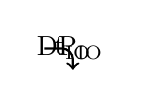
\begin{tikzpicture}
%%\begin{scope}
\tikzset{level 1+/.style={sibling distance=.5\baselineskip}}
%%
\Tree  [.HighAgrP \node(x){DP\textsubscript{IO}}; [ HighAgr [.{...} [.\eee{v}P DP\textsubscript{causer} [ \eee{v}\textsubscript{cause}    [.ApplP \node(v){t\textsubscript{IO}}; {...}  ]]]]]]
%%
\draw[thick,<-,rounded corners] (x.south) |- (v.west);
\end{tikzpicture}
\end{figure}

Reconstruction of the raised subject to this low Spec,\eee{v}\textsubscript{cause} position should thus allow for ``backwards'' binding from the object into the subject, whereas it will continue to be impossible with agents, which are too high for any shifted objects to bind into. 

The analysis just outlined may seem to be in direct conflict with the analysis I outlined in \figref{gt:obj1} above for the core Oehrle effects\is{Oehrle effect} cases: why does the causer subject block \isi{object shift} in \figref{gt:obj1} but not in \figref{gt:6yf}? My proposal is that the relevant difference is that in \figref{gt:6yf} the two DPs differ in terms of animacy: in configurations such as (\ref{gt:df4a}--\ref{gt:8us}), the IO is animate, whereas the causer is inanimate (or can be analyzed thus, unlike with an agent\footnote{Examples such as the following would seem to pose a problem for this analysis: 

\xe{ii}{ Her$_i$ political enemies gave [every journalist]$_i$ the impetus to keep investigating.} 

\noindent I assume that the subject here, when analyzed as a causer, can be coerced as an inanimate with a meaning akin to ``the idea/thought of his enemies'', possibly with a silent noun embedding the overt nominal. I presume a similar analysis would obtain for cases such as \eee{we were discussing John}. }), and this difference allows for A-probes to discern between the two and, thus, for A-locality issues to be circumvented with structures such as \figref{gt:6yf}. On the other hand, in \figref{gt:obj1} above, a structure representing the core \isi{Oehrle effect} cases, both the external argument and the shifted DO are inanimate (\eee{*the noise gave a headache to me}), and so Relativized Minimality would not be able to discern between the two in a way that resolves the locality issue.

The idea that subjects and objects would interact with respect to their relative animacy is not a new one of course; some languages restrict certain combinations of subjects and objects according to animacy hierarchies. (\ref{7fh}) is an example from \ili{Chuj} (from \citealt{gt:Deal:2023}): 

\ea \label{7fh}
\ea
\gll Ix-y-il nok' chan winh winak. \\
 \textsc{pfv-A3}-see \textsc{clf} snake \textsc{clf} man \\
\glt `The man saw the snake.'
\ex
\gll *Ix-y-il winh winak nok' chan. \\
\textsc{pfv-A3}-see \textsc{clf} man \textsc{clf} snake \\ 
\glt Intended: `The snake saw the man.'
\z
\z

\noindent Therefore it is plausible, if somewhat novel, in the landscape of English\il{English (Modern)} to claim that animacy features would be involved in a Minimality calculus impacting upon \isi{object shift}. This analysis brings animacy back into the fold as a means to understanding effects on the dative alternation, but by a rather different route than what was taken by \citet{gt:Oehrle:1976} and \citet{gt:Harley:2002a}, where animacy determined whether a given element could be a possessor. 

On the account here, animacy doesn't play a direct role in determining if a given argument can receive one theta role or another, but rather it determines the range of possible crossing paths, and in turn, the range of possible ditransitive derivations allowing \isi{backwards binding}. This is important for a few reasons. \citet{gt:Harley:2015} make it clear that animacy is not required for a given argument to appear as a possessor IO in a DOC; rather, all that matters is that the related possessive predication is well-formed. The  examples in (\ref{poc}--\ref{poi}) from \citet{gt:Harley:2015} demonstrate this. 

\xex{poc}{
\xl{poc1} \#The advertiser gave the car a flyer. 
\xl{poc2}  \#The car has a flyer. 
}

\xex{poi}{
\xl{poi1} The painter gave the house a new coat of paint. 
\xl{poi2} The house has a new coat of paint. 
}

\noindent Similar remarks hold for external arguments. \citeauthor{gt:Folli:2005} (\citeyear{gt:Folli:2005}; \citeyear{gt:Folli:2006}; \citeyear{gt:Folli:2007}) show that agents can be inanimate so long as they have ``teleological capability''; for example, computer programs, machines or other inanimates can receive agent roles, such as in \eee{the kettle whistled}. Thus, it is expected that there is no strong ban on inanimates as the (agentive) subject of PDCs in English\il{English (Modern)}, and that seems correct, as (\ref{dos}) shows. 

\xex{dos}{
\xl{dos1} iCal sent the participants a reminder. 
\xl{dos2} iCal sent a reminder to the participants. 
}

\noindent Thus, animacy may play some role in determining the semantic compatibility of a given DP with a thematic role, but it is not fully determinative of the range of possibilities. On the other hand, animacy on my account does have a role to play in determining the range of possible and impossible derivations where an object crosses the external argument. This possibility arises with causer external arguments, but not with agents, which are merged above HighAgrP and, thus, cannot be crossed by \isi{object shift} independent of animacy considerations. 
\is{causer subjects|)}

\section{Conclusion}

In this chapter I have argued that Oehrle effects\is{Oehrle effect} should be explained not as a side effect of distinct semantic interpretations for DOCs and PDCs. The semantic explanation, which had been taken to support the two-base theory of the dative alternation, struggles to account for the fact that there is no such incompatibility with PDCs in Scottish Gaelic. This sent me in search of a syntactic alternative, one which is capable of handling cross-linguistic variation in the attestation of Oehrle effects\is{Oehrle effect}. The syntactic alternative that I propose appeals to Relativized Minimality and a more articulated syntax for object licensing. Other syntactic analyses may, of course, present themselves, as data is likewise brought into the picture from other languages. The take-home point here, I suggest, is that apparently semantic effects can quite often be given a syntactic reinterpretation, particularly when there are so many syntactic moving parts to take into account. Comparative data is essential to assessing these matters. 

\il{Irish (Modern)|)}
\il{Scottish Gaelic (Modern)|)}

\section*{Acknowledgments}

Many thanks to Gillebr\`ide MacMillan above all for his time and endless patience working with me on the data that feeds into my work on Gaelic. Thanks also to Andrew Carnie for inviting me to contribute to the series, and to the two reviewers, the other editors, the audience members at the FACL talk (especially Heidi Harley), and also audiences at LSA 2024 and Edinburgh, David Adger, Chris Collins, Stephanie Harves, David Pesetsky, Richie Kayne, Alec Marantz, Craig Sailor, and David Willis for discussion of issues that fed into this work. 


\printbibliography[heading=subbibliography,notkeyword=this]
\end{document}
